\subsection{Свойства показательной функции}

\begin{theorem} Докажем свойства показательной функции. Cчитаем $a, b, c \in (0; +\infty)$, если не сказано обратного.
\begin{table}[h]
\begin{tabular}{cll}
1. & $a^x$~---~строго возрастает & $a \in (1; +\infty)$ \\ 
2. & $a^x$~---~строго убывает & $a \in (0, 1)$ \\
3. & $a^x > 0$ & $\forall x \in \R$ \\
4. & $a^x \cdot a^y = a^{x + y}$ & $\forall x, y \in \R$ \\
5. & $(a^x)^y = a^{xy}$ & $\forall x, y \in \R$ \\
6. & $(bc)^x = b^x \cdot c^x$ & $\forall x \in \R$ \\
7. & $a^x \in \text{C} \big( \R \big)$ & (доказали используя третье) \\
\end{tabular}
\end{table}
\end{theorem}

\begin{proof} 

1. Докажем первое свойство, $a \in (1; +\infty)$, второе анологично. Возьмём $x, y \in \R$: $x < y$.

Так как $x < y \Rightarrow \exists p, q \in \Q$: $\ p \geq x$ и $ q \leq y$: $x < p < q < y.$
    
Возьмем последовательность $\{r_{n}'\} \subset \Q$: $\lim\limits_{n\to \infty} r_{n}' = x$. Тогда $x \leq r_n' \leq p  \ \forall n \in \N.$
        
Возьмем последовательность $\{r_{n}''\} \subset \Q$: $\lim\limits_{n\to \infty} r_{n}'' = y$. Тогда $q \leq r_n'' \leq y \ \forall n \in \N.$
        
Пользуясь свойством монотонности $a^r$ по $r \in \Q$ \newline
        
$a^{x} := \lim\limits_{n \to \infty} a^{r_{n}'}$, $a^{y} := \lim\limits_{n \to \infty} a^{r_{n}''}$.
    
$a^{r_{n}'} \leq a^{p} < a^{q} \leq a^{r_{n}''} \ \forall n \in \N$
    
Из предельного перехода в неравенствах и используя определения $a^x$ и $a^y$ получаем:
    
$$ 
\left\{
\begin{array}{l}
    a^x \leq a^p\\ 
    a^q \leq a^y
\end{array}
\right.
\ \Rightarrow a^x \leq a^p < a^q \leq a^y
$$
    
2. Докажем третье свойство:
    
$a > 1$, $a \in (0, 1)$ аналогично
    
Пусть $x \in \R$. Тогда $\exists p \in \Q: p \leq x$, но для любого рационального числа: $0 < a^p \leq a^x.$

3. Докажем четвертое свойство:
    
Пусть $x, y \in \R.$ Возьмем аппроксимирующие последовательности:
$$\{r_{n}'\}, \{r_{n}''\} \subset \Q : \lim\limits_{n\to \infty} r_{n}' = x, \  \lim\limits_{n\to \infty} r_{n}'' = y .$$
    
$a^{r_n'}\cdot a^{r_n''} = a^{r_n' + r_n''}, \forall n \in \N$
    
Переходим к пределу в равенстве:
    
$a^{x}\cdot a^{y} = a^{x + y}$
    
Так как $x$ и $y$ - произвольные, верно для всех

4. Докажем пятое свойство:
Фиксируем произвольные $x,y \in \R$
Возьмем две аппроксимирующие последовательности для x \newline
Обозначим $r_{n}' \downarrow x, \ , n \to \infty$ Последовательность $r_n'$ монотонно убывает к $x$
    
Обозначим $r_{n}'' \uparrow x, \ , n \to \infty$ Последовательность $r_n''$ монотонно возрастает к $x$
    
$\rho_{n}' \uparrow y, \ n \to \infty$
    
$\rho_{n}'' \uparrow y, \ n \to \infty$
    
$$(a^{r_{n}''})^{\rho_{n}''} \leq (a^{x})^{\rho_{n}''} \leq (a^{x})^{y} \leq (a^{r_{n}'})^{y} \leq a^{r_{n}' \cdot \rho_{n}'}$$
    
В итоге 
    
$$(a^{r_{n}''})^{\rho_{n}''} \leq (a^{x})^{y} \leq a^{r_{n}' \cdot \rho_{n}'}$$
    
Переходим к переделу при $n \to \infty$ в этих двух неравенствах
    
$$a^{x \cdot y} \leq (a^{x})^{y} \leq a^{x \cdot y} \Rightarrow (a^{x})^{y} = a^{x \cdot y}$$

5. Шестое свойство доказывается также предельным переходом

$\{r_{n}'\} \subset \Q : \quad r_{n}' \to x, n \to \infty$
    
$$(bc)^x = \lim\limits_{n \to \infty} (bc)^{r_n'} = \lim\limits_{n \to \infty} b^{r_n'}c^{r_n'} = \lim\limits_{n \to \infty} b^{r_n'} \cdot \lim\limits_{n \to \infty} c^{r_n'} = b^x c^x$$

6. Седьмое свойство (о непрерывности) доказано.

\end{proof}

\begin{definition}
Если в показательной функции $a = e$, то функция вида $e^x$ называется экспонентой
\end{definition}

\begin{definition}
Пусть $a > 0, a \neq 1$, тогда существует обратная функия к $a^x$, называется логарифмом и записывается как $\log_a x$
\end{definition}

\begin{note}
Если $a = 1$ разрешить, то теряется инъективность. Так как $1^x$ это константа, которая отображает все $x$ в одну точку.
\end{note}

\begin{theorem} 
Если $a > 1$, то $\log_a x$ корректно определена, строго возрастает и непрерывна нa луче $(0, +\infty)$, а ее область значений~---~$\R$; 

Если $a \in (0, 1)$ то $\log_a x$ корректно определена, строго убывает и непрерывна н луче $(0, +\infty)$, а ее область значений~---~$\R$.
\end{theorem}

\begin{proof}  
Докажем при $a > 1$, при $a \in (0, 1)$, аналогично.

Так как $a^x$ - строго возрастает и непрерывна, то существует обратная к ней

Область значений луч $(0, +\infty)$

При  $n \in \N$, $a^n \geq 1 + (a - 1)n \to + \infty, \ n \to + \infty$ 

$a^{-n} = \frac{1}{a^n} \leq \frac{1}{(a - 1)n} \to + 0, \ n \to + \infty$ 

$\underset{x \in \R}{\inf} a^x = 0$


$\underset{x \in \R}{\sup} a^x = + \infty$

По обобщенной теореме о промежуточном значении для $a^x$ и теоремы об обратной функции. $\log_a x$ -непрерывен строго возратает на луче $(0, +\infty)$, и область значений $\R$
\end{proof}

\begin{definition}
$ln x := \log_e x$ и называется натуральным логарифмом
\end{definition}

\begin{definition}
    Пусть $\alpha \in \R$. Рассмотим функцию:
    $$ x^{\alpha} := e^{\alpha ln x}, \ x> 0
    $$
    Эта функция строго монотонна (за исключением случая $\alpha = 0$). Она непрерывна на луче $(0, +\infty)$ как композиция непрерывных функций.
    
    Если $\alpha \geq 0$, то $x^{\alpha}$ можно рассмотреть на луче $[0, +\infty),$ полагая $0^{\alpha} := 0$
\end{definition}

\begin{theorem} 
Доказательство некоторых школьных свойства логарифма по определению
\begin{enumerate}
    \item $\log_a xy = \log_a x + \log_a y, \ a > 0, a \neq 1, \ \forall x,y > 0$
    \item $\log_{a} b \cdot \log_{b} a = 1 \quad a > 0, a \neq 1, \quad b> 0, b\neq 1$
    \item $\log_{a} x^{\alpha} = \alpha \log_{a} x, \ x > 0, a> 0, a\neq 1, \alpha \in \R$
\end{enumerate}
\end{theorem}

\begin{proof}  

\begin{enumerate}
    \item Фиксируем произвольные $x, y$, по определнию логарифма (обратная функция):
    $$xy = a^{\log_{a}(xy)}$$

    $$a^{ \log_a x + \log_a y } = (a^{ \log_a x})(a^{ \log_a y}) = xy = a^{ \log_a x}$$

    Так как $a^{x}$ инъективно
    
    $$a^{\log_{a}(xy)} = a^{\log_{a} x + \log_{a} y} \Rightarrow \log_{a} xy = \log_{a} x + \log_{a} y$$
    \item В силу инъективности $a^{x}$
    $$a^{\log_{a}b \cdot \log_{b} a} = \left( a^{\log_{a} b}\right)^{\log_{b} a} = b^{\log_{b} a} = a = a^{1}$$
    \item  $a^{\log_{a} x^{\alpha}} = x^{\alpha}$
    
    $
        a^{\alpha \log_{a} x} =\left(a^{\log_{a} x}\right)^{\alpha} = x^{\alpha}
    $
\end{enumerate}
\end{proof}

\subsection{Второй замечательный предел}
\begin{lemma}
     Пусть $\{n_{k}\}\subset \N$~---~ последовательность натуральных числел, такая что $\exists \lim\limits_{k \to \infty} n_{k} = +\infty$. Тогда:
     $$
     \exists \lim\limits_{k \to \infty} = \left( 1 +\cfrac{1}{n_{k}}\right)^{n_{k}} = e
     $$
\end{lemma}
\begin{proof}
    По определению числа $e$:
    $$
    \forall \epsilon > 0 \ \exists N(\epsilon) \hookrightarrow \left( 1 + \cfrac{1}{n}\right)^{n} \in U_{\epsilon}(e)
    $$

    Так как $\lim\limits_{k \to \infty} n_{k} = +\infty$, то $\exists K(\epsilon): \forall k \geq K(\epsilon) \hookrightarrow n_{k} \geq N(\epsilon) \Rightarrow$

    $$ \Rightarrow\forall \epsilon > 0 \ \exists K(\epsilon): \forall k \geq K(\epsilon) \hookrightarrow \left(1 + \cfrac{1}{n_{k}}\right)^{n_{k}} \in U_{\epsilon}(e) \Rightarrow \exists \lim\limits_{k \to \infty} = \left( 1 +\cfrac{1}{n_{k}}\right)^{n_{k}} = e$$
\end{proof}

\begin{lemma}
    $\exists \lim\limits_{x \to 0+0} \left( 1 + x \right)^{^1/_x} = e$
\end{lemma}
\begin{proof}
    Возьмем последовательность Гейне в нуле (справа) $\{x_{k}\}$, то есть 
    
    $x_{k} \to 0, k\to \infty$ и $x_{k} > 0 \ \forall k \in \N$

    Так как $x_{k} \to +0, k \to \infty \Rightarrow \exists K_{0} \in \N: \ \forall k \geq K_{0} \hookrightarrow x_{k} \in (0, 1) \Rightarrow$

    $$
    \Rightarrow \forall k \geq K_{0} \ \exists n_{k} \in \N: \ (x_{k})^{-1} \in [n_{k}, n_{k+1})
    $$

    $$
     \left(1 + \cfrac{1}{n_{k}+1}\right)^{n_{k}}\leq \left( 1 + x \right)^{^1/_{x_{k}}} \leq \left(1 + \cfrac{1}{n_{k}}\right)^{n_{k}+1}
    $$

    $$
    \left(1 + \cfrac{1}{n_{k}+1}\right)^{n_{k}} = \cfrac{\left(1 + \cfrac{1}{n_{k}+1}\right)^{n_{k}+1}}{1 + \cfrac{1}{n_{k} + 1}} \to e, k \to \infty \ \textrm{по предыдущей лемме}
    $$
    
    $$
    \left(1 + \cfrac{1}{n_{k}}\right)^{n_{k}+1} \to e, k \to \infty \ \textrm{аналогично предыдущему}
    $$

    Так как последовательность Гейне была выбрана произвольно, то вышенаписанное справедливо для любой последовательности Гейне, значит, по теореме об эквивалетности определений по Коши и по Гейне для одностороннего предела функции (аналогична \hypertarget{thm4.1}{ теореме об эквивалетности определений по Коши и по Гейне для предела функции}) получаем $\exists \lim\limits_{x \to 0+0} \left( 1 + x \right)^{^1/_x} = e$
\end{proof}

\begin{lemma}
    $\exists \lim\limits_{x \to 0-0} \left( 1 + x \right)^{^1/_x} = e$
\end{lemma}
\begin{proof}
    Возьмем последовательность Гейне $\{x_{k}\}$ такую, что  
    $x_{k} \to 0, k\to \infty$ и $x_{k} < 0 \ \forall k \in \N$

    Рассмотрим последовательность $y_{k} = \cfrac{-x_{k}}{1+x_{k}} > 0  \Rightarrow x_{k} = \cfrac{-y_{k}}{1+ y_{k}}$

    $$
    (1+x_{k})(1+y_{k}) = 1 \ \forall f \in \N
    $$

    $$
    (1 + x_{k})^{^1/_{x_{k}}} = \Bigl[ (1 + y_{k})^{-1} \Bigr]^{-\cfrac{1 + y_{k}}{y_{k}}} = (1 + y_{k})^{\frac{1}{y_{k}} + 1} = (1 + y_{k})^{\frac{1}{y_{k}}} \cdot (1 + y_{k}) \to e, k \to \infty
    $$
    $$
    (1 + y_{k})^{\frac{1}{y_{k}}} \to e, k \to \infty, \quad \quad  (1 + y_{k}) \to 1, k\to \infty
    $$

    Следовательно, $\exists \lim\limits_{k \to \infty} \left( 1 + x_{k} \right)^{^1/_{x_{k}}} = e$. Значит, $\exists \lim\limits_{x \to 0-0} \left( 1 + x \right)^{^1/_x} = e$.
\end{proof}

\begin{corollary}
    $\exists \lim\limits_{x \to 0} \left( 1 + x \right)^{^1/_x} = e$~---~ \textit{второй замечательный предел}
\end{corollary}

\begin{example}
    $\lim\limits_{x\to 0 } \cfrac{\ln(1 + x)}{x}$ = 1

    $$ \cfrac{\ln (1+x)}{x} = \ln (1 + x)^{^1/_x}$$

    $y (x) = (1 + x)^{^1/_x} $ корректно определена в проколотой окрестности 0, $ \exists \lim\limits_{x \to 0} y(x) = e$

    $\ln(y)$ непрерывна на всей числовой прямой, в частности непрерывна в точке $e$. 
    
    Значит, \hyperlink{thrm4.18}{по теореме о замене переменной при вычислении предела} 
    
    $$\exists \lim\limits_{x \to 0} \ln(y(x)) = \lim\limits_{y \to e} \ln (y) = \ln e = 1$$
\end{example}

\begin{example}
    $ \lim\limits_{x \to 0} \cfrac{e^{x} - 1}{x} = 1$

    $$ 
    \begin{gathered}
        y(x) = e^{x} - 1
    \\
        x = \ln(1 + y(x))  
    \end{gathered}
    \Rightarrow 
    \cfrac{e^{x} - 1}{x} = \cfrac{y(x)}{\ln(1 + y(x))}
    $$

    Так как $e^{x}$ строго растет, то $e^{x} - 1$ тоже. Значит, $y(x)$~---~ инъекция. Следовательно, если $x \neq 0,$ то  $y(x) \neq 0 \Rightarrow \forall x \in \mathring{U}_{\delta}(0) \hookrightarrow y(x) \neq 0$. 
    
    Значит, можно воспользоваться \hyperlink{thrm4.17}{теоремой о замене переменной при вычислении предела}:

    $$
    \exists \lim\limits_{x \to 0} \cfrac{y(x)}{\ln(1 + y(x))} = \lim\limits_{y \to 0} \cfrac{y}{\ln (1+y)} = 1
    $$
\end{example}

\subsection{Эквивалентность функций}

\begin{definition}
    Пусть $\delta_{0} > 0, \ x_{0} \in \overline{\R}$. Пусть $ \begin{gathered}
        f: \mathring{U}_{\delta_{0}}(x_{0}) \mapsto \R, \\
        g:\mathring{U}_{\delta_{0}}(x_{0}) \mapsto \R,
    \end{gathered}$ 
    
    Будем говорить, что $f(x) \sim g(x),\  x\to x_{0},$ если $\exists \theta$:  $\mathring{U}_{\delta_{0}}(x_{0}) \mapsto \R,$ такая что \begin{enumerate}
        \item $\lim\limits_{x \to x_{0}} \theta(x)= 1$;
        \item $f(x) = \theta(x) \cdot g(x) \quad \forall x \in \mathring{U}_{\delta_{0}}(x_{0}).$
    \end{enumerate}
\end{definition}

\begin{definition}
    \hypertarget{def4.40}{\textit{(Из стандартных книжек)}}.

    $f(x) \sim g(x), x\to x_{0},$ если $\exists
     \lim\limits_{x \to x_{0}} \cfrac{f(x)}{g(x)} = 1$, $g (x) \neq 0 \ \forall x \in \R$.
\end{definition}

\begin{note}
    <<$\sim$>>~---~действительно отношения эквивалентности на множестве функций, заданных в $\mathring U_{\delta_{0}}(x_{0}).$
    \begin{enumerate}
        \item[a)] Рефлексивность:  $f(x) \sim f(x), x\to x_{0}$ 
        
    \begin{proof}
        Возьмём $\theta \equiv 1$.
    \end{proof}
        \item[b)] Симметрия: $f(x) \sim g(x)$, $x\to x_{0} \Rightarrow g(x) \sim f(x)$, $x\to x_{0}.$
    \begin{proof}
        $f(x) \sim g(x)$, $x\to x_{0} \Rightarrow \exists \theta(x): \left\{ \begin{gathered}
        \lim\limits_{x \to x_{0}} \theta(x)= 1 \hfill \\
        f(x) = \theta(x) g(x) \hfill
        \end{gathered} \right.$ 

        Тогда пусть $\overline{\theta}(x) = \left\{ \begin{gathered}
            \cfrac{1}{\theta(x)}, \ \theta(x)\neq 0 \hfill \\
            1, \ \theta (x) =  0 \hfill
        \end{gathered} \right.
        \Rightarrow \left\{
        \begin{gathered}
        \lim\limits_{x\to x_{0}} \overline{\theta}(x) = 1 \hfill \\
        g(x) = \overline{\theta }(x) f(x) \quad \forall x\in \mathring{U}_{\delta_{0}}(x_{0}) 
        \end{gathered} \right.$
    \end{proof}
            \item[c)] Транзитивность: $f(x) \sim g(x), x\to x_{0} \ \textrm{и}\ g(x) \sim h(x),  x\to x_{0} \Rightarrow f(x) \sim h(x), x\to x_{0}$

    \begin{proof}
        $
        \begin{gathered}
            \exists \theta_{1}(x): \ f(x) = \theta_{1}(x) g(x) \\
            \exists \theta_{2}(x): \ g(x) = \theta_{2}(x) h(x) \\
            \lim\limits_{x \to x_{0}}\theta_{1}(x)= \lim\limits_{x \to x_{0}}\theta_{2}(x)= 1
        \end{gathered} 
        \Rightarrow \theta(x): = \theta_{1}(x)\theta_{2}(x),
        $
        
        Так как $
        \left\{ \begin{gathered}
        \lim\limits_{x \to x_{0}} \theta(x)= 1 \hfill \\
        f(x) = \theta(x) h(x) \quad \forall x\in \mathring{U}_{\delta_{0}}(x_{0})\hfill
        \end{gathered} \right.
        \Rightarrow
        f(x) \sim h(x), x\to x_{0}
        $      
    \end{proof}
    \end{enumerate}
\end{note}


\sidefig(10 cm)(7 cm)
{
\begin{flushleft}
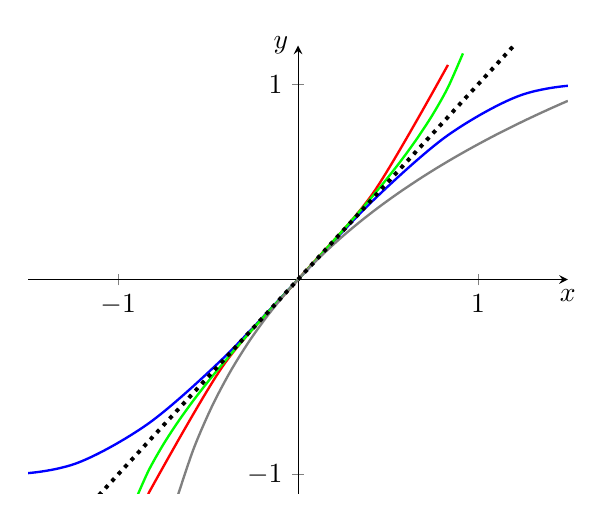
\begin{tikzpicture}[>=stealth][scale = 0.85]
    \begin{axis}[
	axis x line=center,
	axis y line=center,
	xlabel={$x$},
	ylabel={$y$},
	xtick distance=1,
	ytick distance=1,
	xlabel style={below},
	ylabel style={left},
	xmin=-1.5,
	xmax=1.5,
	ymin=-1.1,
	ymax=1.2,
	smooth,
	restrict y to domain=-1.5:1.5,    % <-- added
	]
	\addplot [domain=pi/2:3*pi/2,thick]         {tan(deg(x))};
			\addplot[line width =.03cm,color = blue]  {sin(deg(x))};
			\addplot[line width =.03cm, color = red]  {tan(deg(x))};
			\addplot[line width =.03cm,domain=-1:1,green] {asin(x)/180*pi};
			\addplot[line width =.03cm,color = gray,domain=-1:1.5]  {ln(1+x)};
			\addplot[line width =.05cm, dotted]  {x};
		\end{axis}
\end{tikzpicture}

\end{flushleft}
}
{
\normalsize
\begin{examples} $\ $
\begin{enumerate}
    \item $\sin x \sim x, \ x\to 0$
    \item $\cos x \sim 1,\ x\to 0$
    \item $\tan x \sim x,\ x \to 0$
    \item $\arcsin x \sim x,\ x \to 0$
    \item $e^{x} \sim 1+x,\ x\to 0$
    \item $\ln(1+x) \sim x,\ x\to 0$
\end{enumerate}
\end{examples}
}
    


\begin{lemma}
    Пусть $x_{0} \in \overline{\R}, \ \delta_{0} > 0 \quad f_{1},\ f_{2},\ g_{1},\ g_{2}$: $\mathring{U}_{\delta_{0}}(x_{0}) \mapsto \R \leftarrow$ но так писать не следует, лучше каждую отдельно.

    Пусть $\left\{
    \begin{gathered}
        f_{1}(x) \sim g_{1}(x),\  x\to x_{0} \\
        f_{2}(x) \sim g_{2}(x),\  x\to x_{0}
    \end{gathered} \right.$, тогда $f_{1}(x) \cdot f_{2} (x) \sim g_{1}(x) \cdot g_{2} (x), x\to x_{0}$.

    Если дополнительно $f_{2}(x) \neq 0,\  g_{2}(x) \neq 0, \ \forall x\in \mathring{U}_{\delta_{0}}(x_{0}),$ тогда $\cfrac{f_{1}(x)}{f_{2}(x)} \sim \cfrac{g_{1}(x)}{g_{2}(x)}$, $x\to x_{0}$.
\end{lemma}
\begin{proof}
    $f_{i}(x) \sim g_{i}(x), x\to x_{0} \Rightarrow $
    
    $$
    \Rightarrow \ i =1, 2\quad  \exists \theta_{i}(x): \left\{
    \begin{gathered}
        \lim\limits_{x\to x_{0}} \theta_{i}(x) = 1 \hfill \\
        f_{i}(x) = \theta_{i}(x) g_{i}(x) \quad \forall x\in \mathring{U}_{\delta_{0}}(x_{0}), 
    \end{gathered} \right.$$

    $$
    \theta(x) = \theta_{1}(x)\theta_{2}(x): 
    \left\{ \begin{gathered}
        \lim\limits_{x \to x_{0}} \theta(x)= 1 \hfill \\
        f_{1}(x)f_{2}(x) = \theta(x) g_{1}(x)g_{2}(x) \quad \forall x\in \mathring{U}_{\delta_{0}}(x_{0})\hfill
        \end{gathered} \right.
        \Rightarrow
    $$
    $$
    \Rightarrow
        f_{1}(x)f_{2}(x)\sim g_{1}(x)g_{2}(x), x\to x_{0}
    $$

    Для частного рассуждения аналогичны.
\end{proof}

\begin{note}
    Если $\left\{
    \begin{gathered}
        f_{1}(x) \sim g_{1}(x), x\to x_{0} \\
        f_{2}(x) \sim g_{2}(x), x\to x_{0}
    \end{gathered} \right.$, то из этого \textbf{не} следует, что $f_{1}(x) \pm f_{2} (x) \sim g_{1}(x) \pm g_{2} (x)$, $x\to x_{0}$
\end{note}

\begin{example}
    Возьмём $x^{3} + x \sim x + x^{2}$, $x \to 0$ и $x \sim x$, $x \to 0$. 
    
    Вычтем одно из другого. Неверно, что  $x^{3}\sim x^{2}$, $x\to 0$. 
\end{example}
\begin{note}
    Эквивалентность исходных функций в $\mathring{U}_{\delta_{0}} (x)$ доказывается легко по \hyperlink{def4.40}{<<книжному>> определению}.
\end{note}

Замена на эквивалентность позволяет относительно легко вычислять пределы.

\textit{Примера не будет. Автор устал((}

\begin{lemma}
    Пусть $\delta_{0} > 0, \ x_{0} \in \overline{\R}$. Пусть $ \begin{gathered}
        f: \mathring{U}_{\delta_{0}}(x_{0}) \mapsto \R, \\
        g:\mathring{U}_{\delta_{0}}(x_{0}) \mapsto \R
    \end{gathered}\ $ и $f(x) \sim g(x), x\to x_{0}$ 

    Тогда $\exists \lim\limits_{x\to x_{0}} f(x_{0}) \in \overline{\R} \Leftrightarrow \exists \lim\limits_{x\to x_{0}} g(x)\in \overline{\R}$ и если они оба существуют, то равны.
\end{lemma}
\begin{proof}
    Задание на дом)
\end{proof}

\begin{definition}
    (о-малое) Пусть $\delta_{0} > 0, \ x_{0} \in \overline{\R}$. Пусть $f, g: \mathring{U}_{\delta_{0}}(x_{0}) \mapsto \R$.

    Говорят, что $f$ является \textit{бесконечно малой функцией по сравнению с $g$ при $x \to x_{0}$}, и записывается это как $f(x) = o(g(x)), x \to x_{0}$, если $\exists \epsilon (x)$: $\mathring{U}_{\delta_{0}}(x_{0}) \mapsto \R$ такая что:
    \begin{enumerate}
        \item $\epsilon(x) \to 0, x\to x_{0}$;
        \item $f(x) = \epsilon(x)g(x) \quad \forall x \in \mathring{U}_{\delta_{0}}(x_{0})$.
    \end{enumerate}
\end{definition}
\begin{note} 
    $f(x) = o(g(x))$, $x \to x_{0}$ необратимо, то есть нельзя писать $o(g(x)) = f(x)$, потому что $o(g(x))$~---~это не индивидуально взятая функция, а целый класс функций. 
\end{note}

\begin{lemma}
    Пусть $\delta_{0} > 0$, $x_{0} \in \overline{\R}$. Пусть $f, g$: $\mathring{U}_{\delta_{0}}(x_{0}) \mapsto \R$. Тогда если $f(x) \sim g(x), x\to x_{0}$, то $f(x) - g(x) = o(g(x))$, $x\to x_{0}$.
\end{lemma}
\begin{proof}
    $$\exists \theta(x): \left\{
    \begin{gathered}
        o(x) = 1 \hfill \\
        f(x) = \theta(x) g(x) \quad \forall x\in \mathring{U}_{\delta_{0}}(x_{0}), 
    \end{gathered} \right. \Leftrightarrow f(x) - g(x) = (\theta(x) - 1)g(x) \Leftrightarrow 
    $$
    $$\Leftrightarrow 
    \epsilon(x) = \theta(x) -1 \to 0, \ x\to x_{0}.$$
\end{proof}

\begin{examples} $\ $
        \begin{enumerate}
        \item $\sin x = x + o(x), \ x\to 0$;
        \item $\cos x = 1 + o(x),\ x\to 0$;
        \item $\tan x = x + o(x),\ x \to 0$;
        \item $\arcsin x = x + o(x),\ x \to 0$;
        \item $e^{x} = 1+x + o(x),\ x\to 0$;
        \item $\ln(1+x) = x + o(x),\ x\to 0$.
    \end{enumerate}
\end{examples}

\begin{definition}
     Пусть $\delta_{0} > 0, \ x_{0} \in \overline{\R}$. Пусть $f, g: \mathring{U}_{\delta_{0}}(x_{0}) \mapsto \R$.

     Будем говорить, что $f$ \textit{ограничена относительно $g$ в окрестности точки $x_{0}$} и записывать $f(x) = O(g(x)), x\to x_{0}$, если 

     $$
     \left\{
     \begin{gathered}
         \exists C > 0: \hfill \\
         \exists \delta \in (0, \delta_{0})
     \end{gathered} \right.
     \quad |f(x)| \leq C|g(x)| \quad \forall x\in \mathring{U}_{\delta} (x_{0})
     $$
\end{definition}
\begin{note} 
    $f(x) = O(g(x)), x \to x_{0}$ необратимо, то есть нельзя писать $O(g(x)) = f(x),$ потому что $O(g(x))$~---~ это не индивидуально взятая функция, а целый класс функций. 
\end{note}

\begin{properties} $\ $
    \begin{enumerate}
        \item $o(f) \pm o(f) = o(f), x\to x_{0}$
        \item $o(f) \cdot o(f) = o(f^{2}), x\to x_{0}$
        \item $O(f) \pm O(f) = O(f), x\to x_{0}$
        \item $O(f) \cdot O(f) = O(f^{2}), x\to x_{0}$
        \item $o(f) \cdot O(g) = o(f \cdot g), x\to x_{0}$
        \item $o(f) \pm O(f) = O(f), x\to x_{0}$
        \item $o(f) \cdot o(g) = o(f\cdot g), x\to x_{0}$
    \end{enumerate}
\end{properties}

\section{Производная функции в точке. Дифференциал. Дифференцируемость}

\begin{definition}
    Пусть $f: U_{\delta_{0}}(x_{0}) \mapsto \R, \ x_{0} \in \R, \delta_{0} > 0.$ \textit{Производной функции $f$ в точке $x_{0}$} называется:

    $$
    \cfrac{df}{dx}(x_{0}) = f'(x_{0}) = \lim\limits_{x \to x_{0}} \cfrac{f(x)- f(x_{0})}{x - x_{0}} \in \overline{\R}
    $$
\end{definition}

\begin{definition}
    Пусть $x_{0} \in \R, \ \delta_{0} > 0 \quad x_{0}, x_{0} + h \in U_{\delta_{0}}(x_{0}).$ \textit{Секущей} называется прямая, проходящая через точки $(x_{0}, f(x_{0}))$ и $(x_{0} + h, f(x_{0} + h))$
\end{definition}

\sidefig(10 cm)(7 cm)
{
\begin{flushleft}
$y_{\textrm{сек.}} [x_{0}, h](x) = f(x_{0}) + \cfrac{f(x_{0} + h) - f(x_{0})}{h}(x-x_{0})$
\end{flushleft}
\normalsize
\begin{note}
    \textit{Геометрический смысл производной}~---~ предельное положение секущей, то есть прямая, тангенс угла наклона которой является пределом тангенсов углов наклона секущих в зависимости от $h$
\end{note}
}
{
\begin{tikzpicture}[>=stealth]
		% Рисуем сетку
\draw[help lines, step=0.25, dotted]
(0,0) grid (4,3);
% Начало координат
\draw[->, thin] (0,0) -- (4.05,0)
node[below] {$x$}; % Ox
\draw[->, thin] (0,0) -- (0, 3.05)
node[left] {$y$}; % Oy

\draw[line width =.05cm](0.5, 1.5) parabola bend (1.5, 1)(3.2, 2.75);

\draw[line width =.03cm] (1.355, 0.5) -- (3.45, 2.9);

\draw[dotted, line width =.03cm] (1.9, 0) -- (1.9, 1.1);
\draw[dotted, line width =.03cm] (3.05, 0) -- (3.05, 2.4);
\draw[dotted, line width =.03cm] (0, 2.4) -- (3.05, 2.4);
\draw[dotted, line width =.03cm] (0, 1.1) -- (1.9, 1.1);

\draw [fill = black] (3.02,2.4) circle (1.5pt);
\draw [fill = black] (1.9,1.1) circle (1.5pt);

\node[below] at (3.05, 0) {$x_{0} + h$};
\node[below] at (1.9, 0) {$x_{0}$};
\node[left] at (0, 2.4) {$f(x_{0} + h)$};
\node[left] at (0, 1.1) {$f(x_{0})$};

\node at (-1,0.5) {$y_{\textrm{сек}}(x_{0},h)$}

\end{tikzpicture}



}


\begin{definition}
    Пусть $f: U_{\delta_{0}}(x_{0}) \mapsto \R, \ x_{0} \in \R, \delta_{0} > 0.$ Будем говорить, что $f$ \textit{дифференцируема в точке $x_{0},$} если $\exists A \in \R: f(x) = f(x_{0}) + A(x-x_{0}) + o(x-x_{0}), x\to x_{0}$
\end{definition}

\begin{theorem}
    Функция $f: U_{\delta_{0}}(x_{0}) \mapsto \R$ дифференцируема в точке $x_{0} \Leftrightarrow f'(x_{0}) \in \R.$ При этом $A = f'(x_{0}).$
\end{theorem}
\begin{proof}
    Функция дифференцируема в точке $x_{0}$ значит:
    $$  f(x) = f(x_{0}) + A(x-x_{0}) + \epsilon(x)(x-x_{0}), \ \forall x \in U_{\delta_{0}}(x_{0}), \ \textrm{и} \ \epsilon \to 0, x \to x_{0} \Leftrightarrow$$
    $$
    \Leftrightarrow \cfrac{f(x)- f(x_{0})}{x - x_{0}} = A  + \epsilon(x), \epsilon \to 0, x \to x_{0} \Leftrightarrow  \lim\limits_{x \to x_{0}} \cfrac{f(x)- f(x_{0})}{x - x_{0}} = A$$
\end{proof}

\begin{definition}
    Пусть $f$ дифференцируема в точке $x_{0}$. Тогда \textit{дифференциалом $f$ в точке $x_{0}$} называется функция $df_{x_{0}}(h) = f'(x_{0})h$

    На практике обычно используют обозначения $df(x_{0}, dx) = f'(x_{0})dx$
\end{definition}

\begin{problem}
    Как связаны условия:
    \begin{enumerate}
        \item $f$ дифференцируема в точке $x_{0}$
        \item $f$ непрерывна в точке $x_{0}$
    \end{enumerate}
\end{problem}
\begin{solution}
    1) $\Leftrightarrow \exists A \in \R$: $f(x) = f(x_{0}) + A(x-x_{0}) + o(x-x_{0}) \to f(x_{0})$, так как $ A(x-x_{0}) \to 0$, $o(x-x_{0}) \to 0$, при $x\to x_{0} \Rightarrow 2)$.

    Из 2) не следует 1). Действительно, дифференцируемость равносильна существованию конечной производной. Следовательно, достаточно предъявить функцию непрерывную в точке, но не имеющую в ней конечной производной. 
    
    Например, $f(x) = |x|$ непрерывна в каждой точке, но в нуле не имеет производной.

    $$f'(0) = \lim\limits_{x\to 0} \cfrac{f(x) - f(0)}{x}$$
    $$
    \cfrac{|x| - 0}{x} = \text{sign}x.$$

    Но $\text{sign}x$ в нуле не имеет предела.
    
     \textbf{Ответ:} из 1) следует 2)
\end{solution}